\documentclass[14pt]{extbook}
\usepackage{multicol, enumerate, enumitem, hyperref, color, soul, setspace, parskip, fancyhdr} %General Packages
\usepackage{amssymb, amsthm, amsmath, bbm, latexsym, units, mathtools} %Math Packages
\everymath{\displaystyle} %All math in Display Style
% Packages with additional options
\usepackage[headsep=0.5cm,headheight=12pt, left=1 in,right= 1 in,top= 1 in,bottom= 1 in]{geometry}
\usepackage[usenames,dvipsnames]{xcolor}
\usepackage{dashrule}  % Package to use the command below to create lines between items
\newcommand{\litem}[1]{\item#1\hspace*{-1cm}\rule{\textwidth}{0.4pt}}
\pagestyle{fancy}
\lhead{Progress Quiz 4}
\chead{}
\rhead{Version C}
\lfoot{9187-5854}
\cfoot{}
\rfoot{Spring 2021}
\begin{document}

\begin{enumerate}
\litem{
Find the equation of the line described below. Write the linear equation as $ y=mx+b $ and choose the intervals that contain $m$ and $b$.\[ \text{Parallel to } 4 x + 7 y = 13 \text{ and passing through the point } (-5, 5). \]\begin{enumerate}[label=\Alph*.]
\item \( m \in [-0.86, -0.39] \hspace*{3mm} b \in [-2.3, -0.2] \)
\item \( m \in [-0.86, -0.39] \hspace*{3mm} b \in [9.1, 10.1] \)
\item \( m \in [-0.07, 0.7] \hspace*{3mm} b \in [6.9, 9.1] \)
\item \( m \in [-2.04, -1.46] \hspace*{3mm} b \in [1.1, 4] \)
\item \( m \in [-0.86, -0.39] \hspace*{3mm} b \in [1.1, 4] \)

\end{enumerate} }
\litem{
First, find the equation of the line containing the two points below. Then, write the equation as $ y=mx+b $ and choose the intervals that contain $m$ and $b$.\[ (-10, 8) \text{ and } (7, -9) \]\begin{enumerate}[label=\Alph*.]
\item \( m \in [-1.8, -0.7] \hspace*{3mm} b \in [16, 21] \)
\item \( m \in [-1.8, -0.7] \hspace*{3mm} b \in [-10, 0] \)
\item \( m \in [-0.1, 2.2] \hspace*{3mm} b \in [-20, -9] \)
\item \( m \in [-1.8, -0.7] \hspace*{3mm} b \in [1, 5] \)
\item \( m \in [-1.8, -0.7] \hspace*{3mm} b \in [-20, -9] \)

\end{enumerate} }
\litem{
Find the equation of the line described below. Write the linear equation as $ y=mx+b $ and choose the intervals that contain $m$ and $b$.\[ \text{Perpendicular to } 4 x - 5 y = 13 \text{ and passing through the point } (-3, 5). \]\begin{enumerate}[label=\Alph*.]
\item \( m \in [-1.57, -0.98] \hspace*{3mm} b \in [-2.21, -0.51] \)
\item \( m \in [-1.57, -0.98] \hspace*{3mm} b \in [6.64, 8.13] \)
\item \( m \in [-1.57, -0.98] \hspace*{3mm} b \in [-0.16, 2.44] \)
\item \( m \in [1, 1.31] \hspace*{3mm} b \in [8.33, 9.55] \)
\item \( m \in [-0.89, 0.05] \hspace*{3mm} b \in [-0.16, 2.44] \)

\end{enumerate} }
\litem{
Write the equation of the line in the graph below in Standard form $Ax+By=C$. Then, choose the intervals that contain $A, B, \text{ and } C$.
\begin{center}
    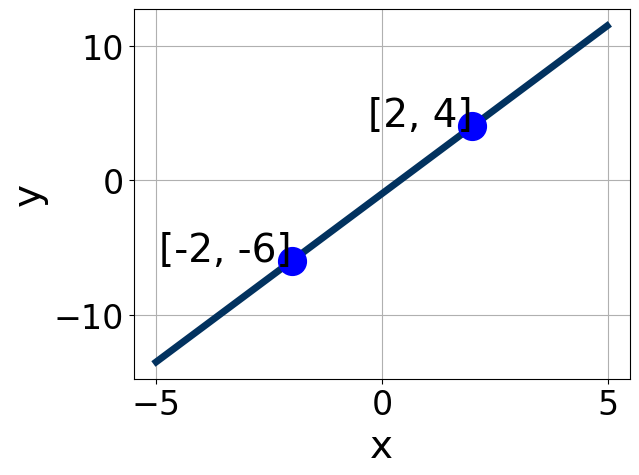
\includegraphics[width=0.5\textwidth]{../Figures/linearGraphToStandardCopyC.png}
\end{center}
\begin{enumerate}[label=\Alph*.]
\item \( A \in [-1.33, 3.67], \hspace{3mm} B \in [-1.32, -0.06], \text{ and } \hspace{3mm} C \in [0.1, 4.5] \)
\item \( A \in [-1.33, 3.67], \hspace{3mm} B \in [0.52, 1.41], \text{ and } \hspace{3mm} C \in [-4.1, -1.6] \)
\item \( A \in [3, 8], \hspace{3mm} B \in [2.44, 3.97], \text{ and } \hspace{3mm} C \in [-6.2, -5.6] \)
\item \( A \in [3, 8], \hspace{3mm} B \in [-3.19, -1.84], \text{ and } \hspace{3mm} C \in [5.1, 9.2] \)
\item \( A \in [-7, -2], \hspace{3mm} B \in [-3.19, -1.84], \text{ and } \hspace{3mm} C \in [5.1, 9.2] \)

\end{enumerate} }
\litem{
Write the equation of the line in the graph below in Standard form $Ax+By=C$. Then, choose the intervals that contain $A, B, \text{ and } C$.
\begin{center}
    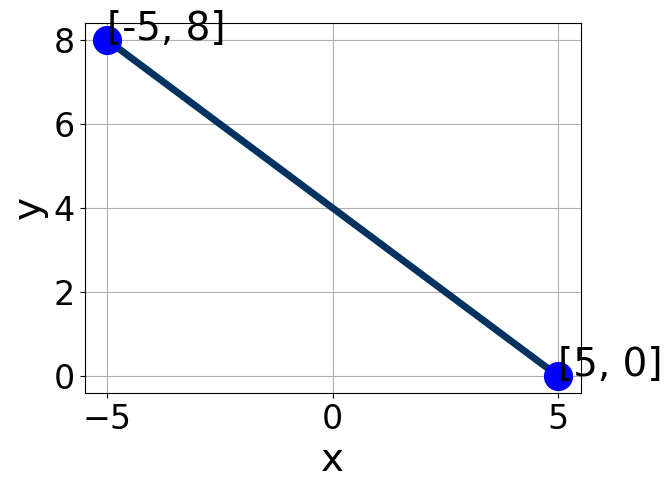
\includegraphics[width=0.5\textwidth]{../Figures/linearGraphToStandardC.png}
\end{center}
\begin{enumerate}[label=\Alph*.]
\item \( A \in [-3.4, -2.4], \hspace{3mm} B \in [-4.7, -1.3], \text{ and } \hspace{3mm} C \in [-20, -12] \)
\item \( A \in [2.7, 3.8], \hspace{3mm} B \in [2.5, 6.3], \text{ and } \hspace{3mm} C \in [14, 17] \)
\item \( A \in [-0.2, 2.1], \hspace{3mm} B \in [0.4, 2.5], \text{ and } \hspace{3mm} C \in [2, 10] \)
\item \( A \in [-0.2, 2.1], \hspace{3mm} B \in [-2, -0.2], \text{ and } \hspace{3mm} C \in [-7, -2] \)
\item \( A \in [2.7, 3.8], \hspace{3mm} B \in [-4.7, -1.3], \text{ and } \hspace{3mm} C \in [-20, -12] \)

\end{enumerate} }
\litem{
Solve the equation below. Then, choose the interval that contains the solution.\[ -5(-17x -6) = -2(19x + 3) \]\begin{enumerate}[label=\Alph*.]
\item \( x \in [-0.33, -0.24] \)
\item \( x \in [-0.56, -0.5] \)
\item \( x \in [0.11, 0.27] \)
\item \( x \in [-0.26, -0.17] \)
\item \( \text{There are no real solutions.} \)

\end{enumerate} }
\litem{
Solve the linear equation below. Then, choose the interval that contains the solution.\[ \frac{-5x + 8}{7} - \frac{-7x + 3}{4} = \frac{8x -3}{8} \]\begin{enumerate}[label=\Alph*.]
\item \( x \in [-0.87, 3.13] \)
\item \( x \in [-228, -223] \)
\item \( x \in [-67.5, -57.5] \)
\item \( x \in [-27.5, -19.5] \)
\item \( \text{There are no real solutions.} \)

\end{enumerate} }
\litem{
Solve the equation below. Then, choose the interval that contains the solution.\[ -2(-6x + 17) = -15(-7x + 5) \]\begin{enumerate}[label=\Alph*.]
\item \( x \in [-1.22, -1.02] \)
\item \( x \in [-0.53, 0.46] \)
\item \( x \in [0.87, 1.1] \)
\item \( x \in [1.04, 1.26] \)
\item \( \text{There are no real solutions.} \)

\end{enumerate} }
\litem{
Solve the linear equation below. Then, choose the interval that contains the solution.\[ \frac{7x -5}{2} - \frac{9x + 7}{7} = \frac{8x -5}{5} \]\begin{enumerate}[label=\Alph*.]
\item \( x \in [10.4, 12.4] \)
\item \( x \in [0.81, 3.81] \)
\item \( x \in [-3.25, 0.75] \)
\item \( x \in [3.07, 7.07] \)
\item \( \text{There are no real solutions.} \)

\end{enumerate} }
\litem{
First, find the equation of the line containing the two points below. Then, write the equation as $ y=mx+b $ and choose the intervals that contain $m$ and $b$.\[ (-2, 4) \text{ and } (-6, 10) \]\begin{enumerate}[label=\Alph*.]
\item \( m \in [-1.5, -0.5] \hspace*{3mm} b \in [-1.1, -0.6] \)
\item \( m \in [0.5, 2.5] \hspace*{3mm} b \in [16.9, 20.9] \)
\item \( m \in [-1.5, -0.5] \hspace*{3mm} b \in [13, 16.5] \)
\item \( m \in [-1.5, -0.5] \hspace*{3mm} b \in [0.5, 3.4] \)
\item \( m \in [-1.5, -0.5] \hspace*{3mm} b \in [5.7, 7.5] \)

\end{enumerate} }
\end{enumerate}

\end{document}